\documentclass[a4paper,12pt]{article}
\usepackage{fancyhdr}
\usepackage{amsmath}
\usepackage{multicol}
\usepackage{verbatim}
\usepackage[pdftex]{graphicx}
\usepackage{float}
\usepackage{hyperref}
\usepackage[left=2cm,top=2cm,right=2cm,nohead,nofoot]{geometry}
%\usepackage{algpseudocode}
\usepackage{float}
\usepackage{caption}
\usepackage{subcaption}
\usepackage{moreverb}
\usepackage{enumerate}
\usepackage{algorithmicx}
\usepackage{graphicx}
\usepackage{amssymb}
\usepackage{color,soul}
\usepackage{soul}

% \usepackage[T1]{fontenc}
% \usepackage[utf8]{inputenc}
% \usepackage{mathptmx}

\pagestyle{empty}


\pagestyle{fancy}
\lhead{\footnotesize {University of Maryland\\CMSC 727: Neural Modeling}}
\rhead{\footnotesize Studying Boosting Techniques in RNNs\\May $9^{th}$, 2017}
\headheight = 50pt
\headsep = 25pt
\textheight = 600pt
\footskip = 30pt

\begin{document}


\begin{center}

\textbf{
Studying Boosting Techniques in RNNs\\
}

{\small Ankit Mondal \quad Sriram Vasudevan \qquad Moustafa Meshry \quad Yancy Liao}\\
{\scriptsize \{amondal2, sriram12\} @ umd.edu \qquad \qquad \qquad \{mmeshry, yliao2\} @ cs.umd.edu}
\end{center}

\section{Abstract}



%==============================================================================


\section{Introduction}


%==============================================================================


\section{Background and related work}


%==============================================================================


\section{Approach}

\subsection{Ensemble learning}

%------------------------------------------------------------------------------
\subsection{Dropout for regularization}
One form of regularization is called dropout, where nodes are "dropped" with a certain probability by setting their values to zero. Dropout may be performed on the input layer, the output layer, or hidden layers, depending on the implementation. Dropout has been shown effective for feedforward networks, but has not met with much success in recurrent neural networks. A previous study showed moderate success with dropout in LSTMs when dropout was restricted to non-recurrent (input/output) layers rather than the recurrent nodes \cite{zaremba2015dropout}.\\

We want to use dropout while training an LSTM on the IMDB dataset. We wish to see whether dropout is effective, and what is the effect of changing the dropout value on the accuracy of the models. Since TFLearn's dropout implementation is also performed on the input/output layers, based on the previous study we predict that dropout should produce moderately increased accuracy around values of 0.5 (maximal randomness) while declining slightly toward 1.0 where effectively there is no dropout, and degrading significantly when approaching 0 when effectively the network is shut down. It should be noted that in the 2015 study of dropout in LSTMs, the authors were using larger models with more complicated multi-class datasets, while tuning other learning parameters, so the results may not generalize here.

%------------------------------------------------------------------------------
\subsection{Adaboost}


%==============================================================================


\section{Experimental results}

\subsection{Datasets}

%------------------------------------------------------------------------------
\subsection{Ensemble learning}

%------------------------------------------------------------------------------
\subsection{Dropout}
We trained TFLearn LSTMs with a learning rate of 0.005 for three separate classes of models according to how many hidden units they had: 4, 64, or 128. With each class of model, we used dropout values ranging from 0.1 (lots of dropout) to 1.0 (no dropout) in increments of 0.1. For each configuration, we trained two models and took their average accuracy. We then plotted the accuracy averages versus dropout values in the figures below, for the three classes.

\begin{figure}[!htb]
	\minipage{0.32\textwidth}
	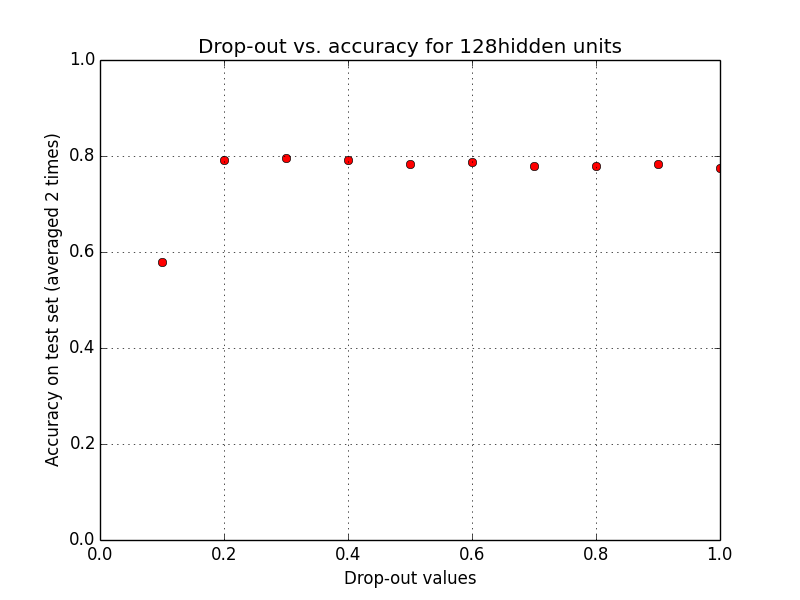
\includegraphics[width=\linewidth]{dropout_plot_128.png}
	\caption{128 hidden units}\label{fig:awesome_image1}
	\endminipage\hfill
	\minipage{0.32\textwidth}
	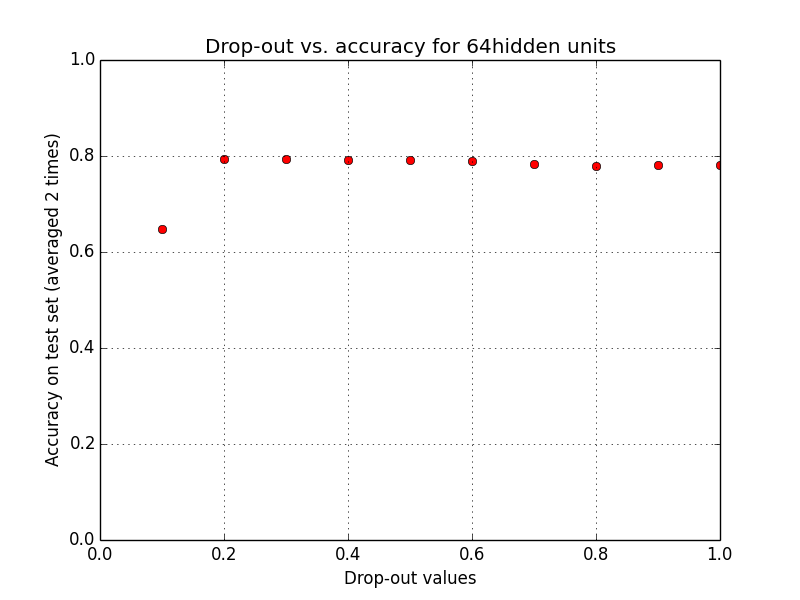
\includegraphics[width=\linewidth]{dropout_plot_64.png}
	\caption{64 hidden units}\label{fig:awesome_image2}
	\endminipage\hfill
	\minipage{0.32\textwidth}%
	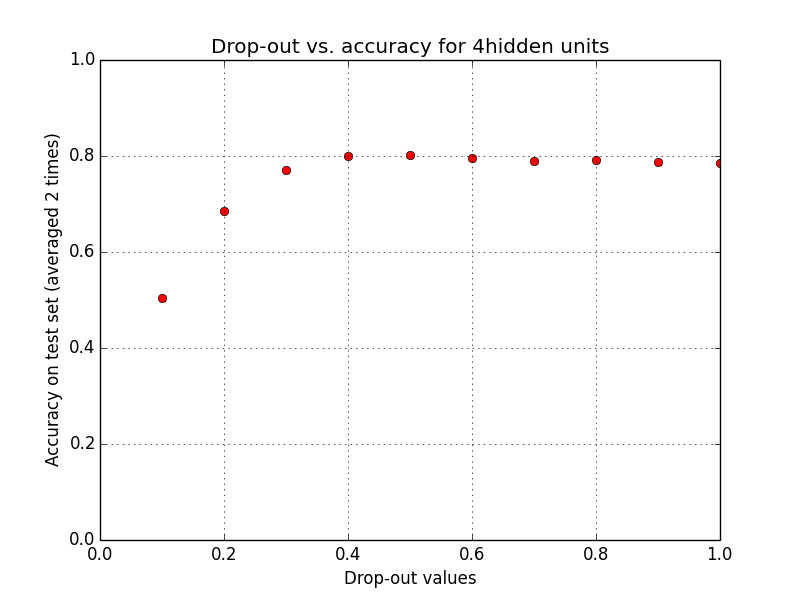
\includegraphics[width=\linewidth]{dropout_plot_4.png}
	\caption{4 hidden units}\label{fig:awesome_image3}
	\endminipage
\end{figure}

In the three cases, our prediction for the efficacy of dropout was not realized. For no values of dropout did the model perform better than the baseline of having no dropout (value of 1.0). Apart from the very clear degradation of accuracy at high amounts of dropout (values of 0.1 or 0.2), we were surprised to find that the dropout values neither improved nor worsened the model accuracy. As one can see from the plots, there is a dip on the far left side of the plots, but then it's relatively flat all the way to the right. 



%------------------------------------------------------------------------------
\subsection{Adaboost}
\subsubsection{Sensitivity analysis}

%------------------------------------------------------------------------------
\subsubsection{IMDB results}

%------------------------------------------------------------------------------

\subsubsection{Char-RNN results}


%==============================================================================


\section{Conclusion}
\label{sec:conclusion}


%==============================================================================

% \pagebreak
{\small
\bibliographystyle{plain}
\bibliography{refs}
}

\end{document}
